\section{Vista Física}
En la siguiente imagen \ref{fig:Diagrama de Despliegue - Vista Física}, se muestra el diagrama de despliegue de la aplicación. Se tienen dos nodos, el primero es la computadora personal ya sea de escritorio o una laptop con cualquier sistema operativo, la única condición es que tenga Java instalado en su última versión para poder ejecutar el fichero 'mantenimiento.jar'. Del lado del servidor, se corre la base de datos que será manipulada por medio del sistema. 
\\
Básicamente se esta siguiendo un Modelo Cliente - Servidor, en este modelo el Cliente realiza peticiones al servidor y se llevan a cabo todas las tareas que se han programado en el sistema. Por otro lado en el Servidor, se encarga de 'escuchar' las peticiones del Cliente para manipular la información almacenados en la base de datos.
\begin{figure}[!h]
	\centering
	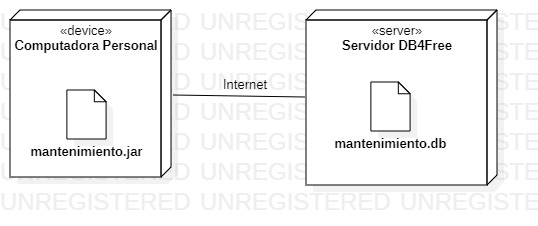
\includegraphics[width=0.8\textwidth]{./diseno/vfisica/imagenes/vistaFisica}
	\caption{Diagrama de Despliegue - Vista Física}
	\label{fig:Diagrama de Despliegue - Vista Física}
\end{figure}